\chapter{Iteracion 6}
\section{Objetivos de iteración}
\begin{itemize}
 \item Integración de documentación de Swagger en la memoria y el proyecto.
 \item Testing, integración contínua
\end{itemize} 

\section{Integración de Swagger}
\subsection{Generar la documentación del API REST}
\emph{Swagger} es una especificación que permite documentar servicios REST. Alrededor de
esta especificación existen multitud de herramientas y proyectos que se encargan de
generar dicha documentación a partir de código o de generar otras formas de consumir la
documentación.

Para nuestro caso la generación de la documentación a partir de código, anotaciones, etcétera
no es posible. El tipo de herramientas que genera la documentación se apoyan en \emph{frameworks} 
con estructuras bien definidas para servicios REST, lo que les permite saber cómo extraer esa 
documentación. \emph{Vert.x} es un \emph{framework} de propósito demasiado general como para que 
exista una herramienta capaz de extraer del código de un servidor \emph{Vert.x} dicha información.

Por tanto nos limitaremos a escribir un archivo \emph{Json} con la documentación del servicio
de forma manual.


\subsection{Consumir la documentación}
Hemos desarrollado dos métodos para hacer que la documentación sea accesible para terceros:

\begin{itemize}
 \item Html en el servidor
 \item PDF en la memoria
\end{itemize}


\subsubsection{Html en el servidor}
El proyecto \emph{Swagger-ui} consiste en una serie de archivos \emph{html} y \emph{javascript}
capaces de leer un archivo de documentación \emph{json} de \emph{Swagger} y mostrarla como
\emph{html}, dando incluso la posibilidad de ejecutar peticiones al servicio basándose en
dicha documentación. Para que funcione sólo es necesario suministrarle la URL del archivo
\emph{Json} con la misma.

Para integrarlo en nuestro servicio hemos escrito un pequeño servidor HTTP que se integra con
nuestro servicio a nivel de \emph{RouteMatcher} y sirve el contenido de \emph{Swagger-ui}
bajo un subdirectorio del servidor (\texttt{/doc/}).


\subsubsection{PDF en la memoria}
Utilizando una combinación de los paquetes \emph{npm} y \emph{Bootprint} de \emph{node.js} y
\emph{PhantomJS} somos capaces de generar primero unos archivos HTML describiendo el servicio
REST y después, a partir de estos, un archivo PDF. Todo el proceso esta automatizado a través
de tareas de \emph{Gradle}, siendo necesaria de forma manual unicamente la instalación de 
\emph{PhantomJS} (un motor \emph{Javascript} ``sin navegador'', \emph{headless}).

Dicho archivo PDF es después incluido en la memoria como anexo.


\section{Testing, Integración contínua}
Tras evaluar el servicio \emph{CircleCI} (\texttt{https://circleci.com/}) hemos decidido utilizarlo.

\emph{CircleCI} sólo nos impone tener como VCS \emph{GIT} de forma accesible. Concretamente esta
muy integrado con la plataforma \emph{Git-Hub}, por lo que hemos mudado el desarrollo del proyecto
a dicha plataforma. La url actual del repositorio es: 
\texttt{https://github.com/andihit/dad-gameregistry.git} 

Los datos generales del proyecto han sido actualizados.

Como resultado de la integración, tras el envío de una nueva revisión a \emph{Git-Hub} este
automaticamente (a traves de un \emph{Post-build-hook}) avisa a \emph{CircleCI} de la nueva
revisión y este a su vez descarga el código, lo compila, ejecuta los tests y guarda el informe.


\section{UML actualizado}

El tamaño del diagrama y la lista de argumentos empieza a ser demasiado como para mostrarlo
entero. Obviando los parámetros de las operaciones, sin embargo, la estructura de clases
actual resulta en el siguiente diagrama.

\begin{figure}[h]
 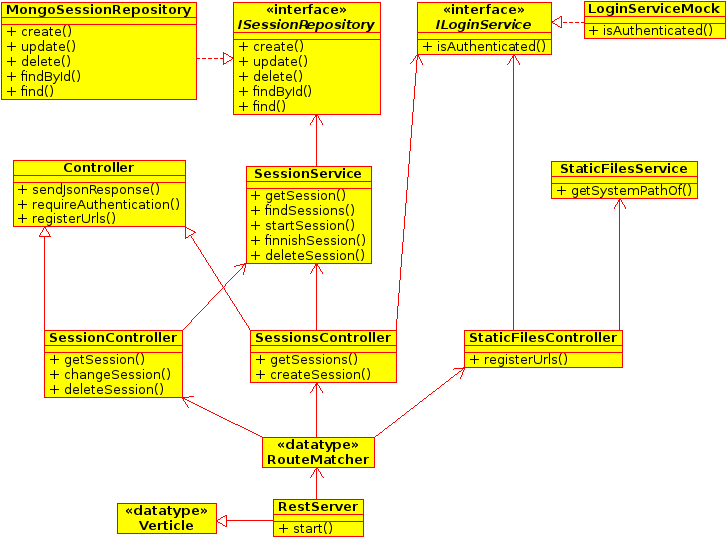
\includegraphics[scale=0.8]{diagrams/class_diagram_iter6.png}
 \caption{Diagrama de clases (iteración 6)}
 \label{fig:clases}
\end{figure} 